\subsection{Análisis descriptivo}
\label{sec:descriptivo}

\subsubsection{Distribución de la eficiencia hidráulica}

La Tabla~\ref{tab:resumen_y} resume la eficiencia hidráulica de las 80 corridas (sección~4 del script). La eficiencia media es de 0.6540, con una desviación estándar de 0.0245 y un coeficiente de variación de 3.74\,\%, es decir, las eficiencias cambian poco en términos relativos. Los valores van de 0.6025 a 0.7165.

Además de la media y la desviación estándar, la tabla incluye tres medidas de la forma de la distribución:

\begin{itemize}[leftmargin=*, itemsep=2pt]
  \item \textbf{Rango intercuartílico (RIQ).} Es la diferencia entre el tercer cuartil ($Q_3$, el valor que deja por debajo al 75\,\% de los datos) y el primer cuartil ($Q_1$, que deja por debajo al 25\,\%): $\text{RIQ} = Q_3 - Q_1$. Mide la amplitud del 50\,\% central de los datos y, a diferencia del rango o la desviación estándar, no se ve afectado por valores extremos. Aquí $Q_1 = 0.6360$ y $Q_3 = 0.6715$, así que la mitad central de las corridas tiene eficiencias en un intervalo de apenas 0.0355.

  \item \textbf{Asimetría.} Mide si la distribución se extiende más hacia un lado que hacia el otro. Se calcula como
  \[
  g_1 = \frac{\frac{1}{n}\sum_{i=1}^{n}(y_i-\bar{y})^3}{s^3}.
  \]
  Vale cero en una distribución simétrica, es positiva cuando la cola derecha es más larga (hay algunos valores altos alejados del resto) y negativa cuando la cola larga está a la izquierda. El valor de 0.380 indica una asimetría leve hacia la derecha: hay algunas corridas con eficiencias altas, cercanas a 0.70, más alejadas de la media que las corridas de eficiencia baja. Por eso la media (0.6540) queda un poco por encima de la mediana (0.6515).

  \item \textbf{Exceso de curtosis.} La curtosis mide qué tan pesadas son las colas de una distribución, es decir, qué tanto pesan los valores muy alejados de la media. Se calcula como $\frac{1}{n}\sum_{i=1}^{n}(y_i-\bar{y})^4 / s^4$, y en una distribución normal vale 3. Por eso se suele reportar el \emph{exceso} de curtosis, que es la curtosis menos 3, de modo que la normal sirva de referencia con un valor de cero. Un exceso positivo indica colas más pesadas que la normal (más valores extremos de lo esperado) y uno negativo, colas más livianas. El valor de $-0.351$ indica que las eficiencias tienen colas algo más livianas que una normal: hay pocos valores muy alejados de la media.
\end{itemize}

\begin{table}[H]
\centering
\caption{Medidas descriptivas de la eficiencia hidráulica ($n = 80$).}
\label{tab:resumen_y}
\begin{tabular}{lc@{\hspace{1.5cm}}lc}
\toprule
Medida & Valor & Medida & Valor \\
\midrule
Media               & 0.6540 & Mínimo                  & 0.6025 \\
Mediana             & 0.6515 & Máximo                  & 0.7165 \\
Desviación estándar & 0.0245 & Rango intercuartílico   & 0.0355 \\
Coef. de variación  & 3.74\,\% & Asimetría             & 0.380 \\
                    &        & Exceso de curtosis      & $-0.351$ \\
\bottomrule
\end{tabular}
\end{table}

La Figura~\ref{fig:distribucion} muestra estas características de forma gráfica. El panel~(a) es un histograma: el rango de eficiencias se divide en 12 intervalos y la altura de cada barra indica cuántas corridas caen en ese intervalo, en escala de densidad (el área total de las barras suma uno). La curva negra es una estimación suavizada de esa densidad y la línea roja discontinua marca la media. Se ve una distribución con un solo pico, alrededor de 0.65, y una cola derecha un poco más larga, lo que coincide con la asimetría positiva.

El panel~(b) es un diagrama de caja. La caja va del primer al tercer cuartil ($Q_1 = 0.6360$ y $Q_3 = 0.6715$), así que su altura es el rango intercuartílico y contiene al 50\,\% central de las corridas; la línea negra dentro de la caja es la mediana. Los bigotes se extienden hasta la corrida más extrema que esté a menos de $1.5 \times \text{RIQ}$ de la caja, es decir, entre 0.5828 y 0.7248; los valores por fuera de esos límites se considerarían atípicos. Los puntos negros son las 80 corridas, separadas un poco en horizontal para que no se superpongan. Ninguna corrida queda por fuera de los bigotes, así que no hay eficiencias atípicas, y la mediana está algo más cerca del borde inferior de la caja, otra señal de la leve asimetría a la derecha.

\begin{figure}[H]
\centering
\begin{minipage}[b]{0.62\textwidth}
  \centering
  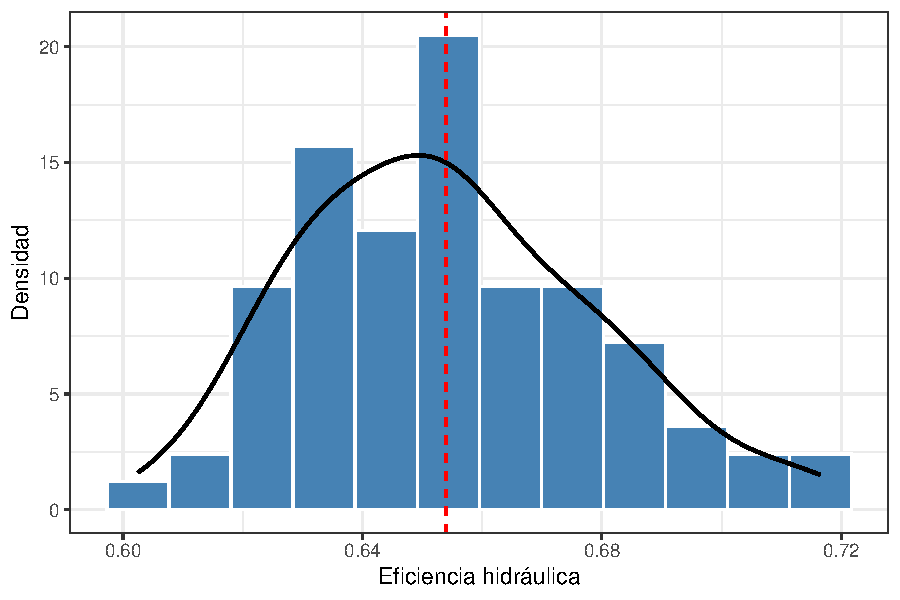
\includegraphics[width=\textwidth]{Articulo_LaTeX/Figs/g1_histograma.pdf}\\[-2pt]
  {\small (a)}
\end{minipage}\hfill
\begin{minipage}[b]{0.35\textwidth}
  \centering
  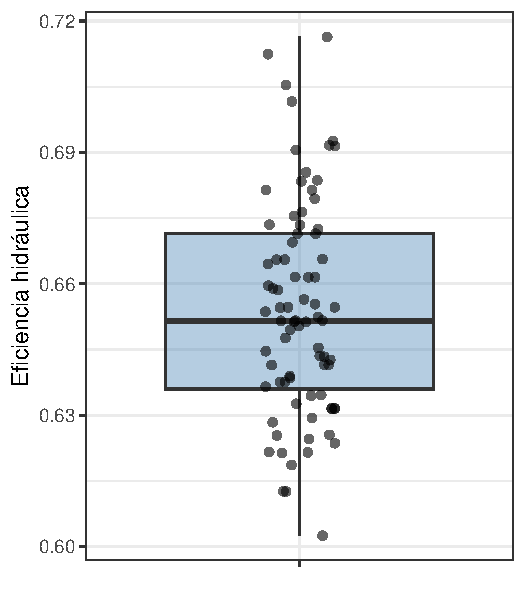
\includegraphics[width=\textwidth]{Articulo_LaTeX/Figs/g2_boxplot.pdf}\\[-2pt]
  {\small (b)}
\end{minipage}
\caption{Histograma con curva de densidad (a) y diagrama de caja (b) de la eficiencia hidráulica. La línea roja discontinua marca la media. Código: sección~4 de \texttt{anal\_descrip.R}.}
\label{fig:distribucion}
\end{figure}

\subsubsection{Eficiencia según cada variable explicativa}

La Tabla~\ref{tab:niveles} y la Figura~\ref{fig:por_variable} muestran la eficiencia según cada variable explicativa (sección~5 del script). En la figura hay un diagrama de caja por cada nivel de cada variable, construido igual que en la Figura~\ref{fig:distribucion}(b) pero solo con las corridas de ese nivel; los puntos azules son las corridas y el rombo rojo es la media del grupo. Si las cajas de los distintos niveles están a alturas diferentes, la variable está asociada con la eficiencia; si se superponen mucho, la diferencia entre niveles es pequeña comparada con la variación dentro de cada nivel. Los niveles medios (92.5°, 12~mm y 50~mm) tienen el doble de corridas que los extremos porque ahí están las réplicas del punto central.

\begin{table}[H]
\centering
\caption{Eficiencia hidráulica según el nivel de cada variable explicativa.}
\label{tab:niveles}
\begin{tabular}{llccccc}
\toprule
Variable & Nivel & $n$ & Media & Desv. est. & Mínimo & Máximo \\
\midrule
\multirow{3}{*}{Ángulo (°)}       & 90    & 21 & 0.6788 & 0.0219 & 0.6285 & 0.7165 \\
                                  & 92.5  & 40 & 0.6478 & 0.0171 & 0.6185 & 0.6915 \\
                                  & 95    & 19 & 0.6394 & 0.0208 & 0.6025 & 0.6835 \\
\midrule
\multirow{3}{*}{Diámetro (mm)}    & 10    & 20 & 0.6618 & 0.0271 & 0.6125 & 0.7165 \\
                                  & 12    & 40 & 0.6507 & 0.0193 & 0.6215 & 0.7055 \\
                                  & 14    & 20 & 0.6527 & 0.0300 & 0.6025 & 0.7125 \\
\midrule
\multirow{3}{*}{Distancia (mm)}   & 40    & 21 & 0.6679 & 0.0260 & 0.6255 & 0.7165 \\
                                  & 50    & 40 & 0.6492 & 0.0188 & 0.6185 & 0.7055 \\
                                  & 60    & 19 & 0.6485 & 0.0282 & 0.6025 & 0.7015 \\
\midrule
\multirow{2}{*}{Rodete}           & Pelton & 40 & 0.6441 & 0.0212 & 0.6025 & 0.6925 \\
                                  & Turgo  & 40 & 0.6638 & 0.0238 & 0.6125 & 0.7165 \\
\midrule
\multirow{2}{*}{Boquillas}        & 1     & 40 & 0.6429 & 0.0211 & 0.6025 & 0.6915 \\
                                  & 2     & 40 & 0.6650 & 0.0227 & 0.6235 & 0.7165 \\
\bottomrule
\end{tabular}
\end{table}

El ángulo de la boquilla es la variable con el efecto más claro: la eficiencia media baja de 0.679 a 90° a 0.639 a 95°, y la caja de 90° está casi por completo por encima de las otras dos. El rodete Turgo es en promedio más eficiente que el Pelton (0.664 frente a 0.644) y usar dos boquillas también aumenta la eficiencia media (0.665 frente a 0.643); en ambos casos las cajas se desplazan hacia arriba, aunque se superponen en parte. Con el diámetro y la distancia la eficiencia media es mayor en el nivel bajo (10~mm y 40~mm), pero las diferencias son menores y las cajas se superponen mucho, porque la dispersión dentro de cada nivel es grande.

\begin{figure}[H]
\centering

\includegraphics[width=0.92\textwidth]{Articulo_LaTeX/Figs/g3_boxplot_por_variable.pdf}
\caption{Eficiencia hidráulica según cada variable explicativa. Los rombos rojos marcan la media de cada grupo. Código: sección~5 de \texttt{anal\_descrip.R}.}
\label{fig:por_variable}
\end{figure}

\subsubsection{Eficiencia media con intervalos de confianza}

Los diagramas de caja muestran cómo se reparten las corridas; para comparar los niveles conviene mirar también qué tan precisa es cada media. La Figura~\ref{fig:medias} muestra la eficiencia media de cada nivel con su intervalo de confianza del 95\,\%, calculado con la distribución $t$ de Student:
\[
\bar{y} \pm t_{0.975,\,n-1}\,\frac{s}{\sqrt{n}},
\]
donde $\bar{y}$, $s$ y $n$ son la media, la desviación estándar y el número de corridas del nivel. Cada punto es una media, las barras son el intervalo y la línea une las medias para mostrar la tendencia. La Tabla~\ref{tab:ic} presenta los mismos intervalos (sección~6 del script).

\begin{figure}[H]
\centering
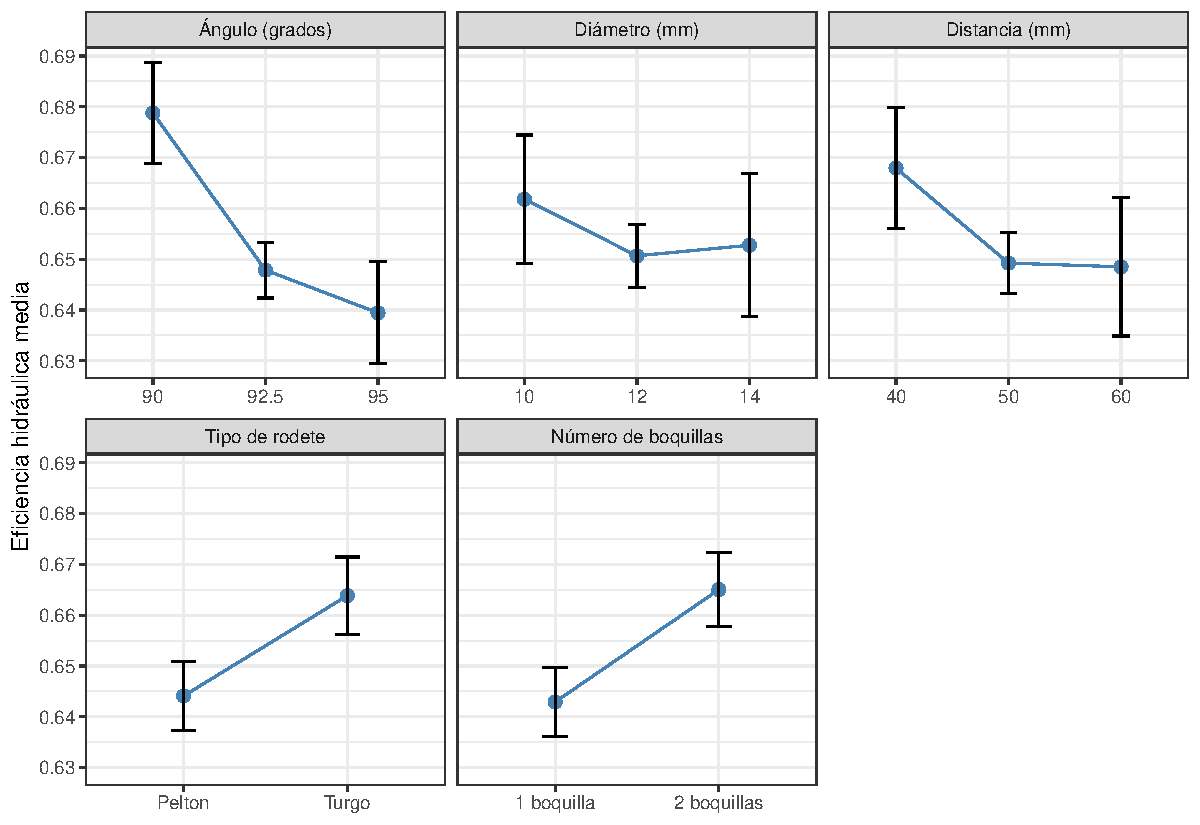
\includegraphics[width=0.92\textwidth]{Articulo_LaTeX/Figs/g4_medias_ic95.pdf}
\caption{Eficiencia media e intervalo de confianza del 95\,\% para cada nivel de cada variable explicativa. Código: sección~6 de \texttt{anal\_descrip.R}.}
\label{fig:medias}
\end{figure}

\begin{table}[H]
\centering
\caption{Eficiencia media e intervalo de confianza del 95\,\% por nivel.}
\label{tab:ic}
\begin{tabular}{llcccc}
\toprule
Variable & Nivel & Media & Límite inferior & Límite superior & Ancho \\
\midrule
\multirow{3}{*}{Ángulo (°)}     & 90     & 0.6788 & 0.6688 & 0.6888 & 0.0200 \\
                                & 92.5   & 0.6478 & 0.6424 & 0.6533 & 0.0109 \\
                                & 95     & 0.6394 & 0.6294 & 0.6495 & 0.0201 \\
\midrule
\multirow{3}{*}{Diámetro (mm)}  & 10     & 0.6618 & 0.6491 & 0.6745 & 0.0254 \\
                                & 12     & 0.6507 & 0.6445 & 0.6569 & 0.0124 \\
                                & 14     & 0.6527 & 0.6387 & 0.6668 & 0.0281 \\
\midrule
\multirow{3}{*}{Distancia (mm)} & 40     & 0.6679 & 0.6561 & 0.6798 & 0.0237 \\
                                & 50     & 0.6492 & 0.6432 & 0.6553 & 0.0121 \\
                                & 60     & 0.6485 & 0.6349 & 0.6621 & 0.0272 \\
\midrule
\multirow{2}{*}{Rodete}         & Pelton & 0.6441 & 0.6373 & 0.6509 & 0.0136 \\
                                & Turgo  & 0.6638 & 0.6562 & 0.6714 & 0.0152 \\
\midrule
\multirow{2}{*}{Boquillas}      & 1      & 0.6429 & 0.6362 & 0.6497 & 0.0135 \\
                                & 2      & 0.6650 & 0.6578 & 0.6723 & 0.0145 \\
\bottomrule
\end{tabular}
\end{table}

Una forma informal de leer la figura es fijarse si los intervalos de dos niveles se superponen. Con el ángulo, el intervalo de 90° $[0.6688;\ 0.6888]$ queda completamente por encima de los de 92.5° y 95°, mientras que estos dos últimos se superponen, así que la caída fuerte ocurre entre 90° y 92.5°. Con el tipo de rodete y el número de boquillas los intervalos no se superponen: el Turgo y el uso de dos boquillas tienen una eficiencia media claramente mayor. Con la distancia, el intervalo de 40~mm apenas queda por encima del de 50~mm (0.6561 frente a 0.6553) y se superpone con el de 60~mm. Con el diámetro, los tres intervalos se superponen, de modo que estos datos no muestran por sí solos una diferencia clara entre diámetros.

Los intervalos de los niveles medios son más angostos (alrededor de 0.011 a 0.012, frente a 0.020 a 0.028 en los extremos) porque tienen el doble de corridas y el ancho del intervalo decrece con $\sqrt{n}$. Hay que tener en cuenta dos cosas al interpretar esta figura. Primero, cada media promedia sobre todos los valores de las demás variables, así que no aísla el efecto de una variable manteniendo las otras fijas; eso lo hace el modelo de regresión. Segundo, que dos intervalos se superpongan no prueba que las medias sean iguales: es solo una guía visual, y la comparación formal se hará con las pruebas del modelo.

\subsubsection{Posibles interacciones}

La Figura~\ref{fig:perfiles} presenta gráficos de perfiles (sección~7 del script). Cada línea corresponde a una combinación de tipo de rodete y número de boquillas, y cada punto es la eficiencia media de las corridas de esa combinación en un nivel de la variable del eje horizontal. Este gráfico sirve para buscar interacciones: si el efecto de una variable es el mismo en todas las combinaciones, las líneas son paralelas y solo se desplazan hacia arriba o hacia abajo; si las líneas tienen pendientes distintas o se cruzan, el efecto de esa variable depende del tipo de rodete o del número de boquillas.

\begin{figure}[H]
\centering
\begin{minipage}[b]{0.49\textwidth}
  \centering
  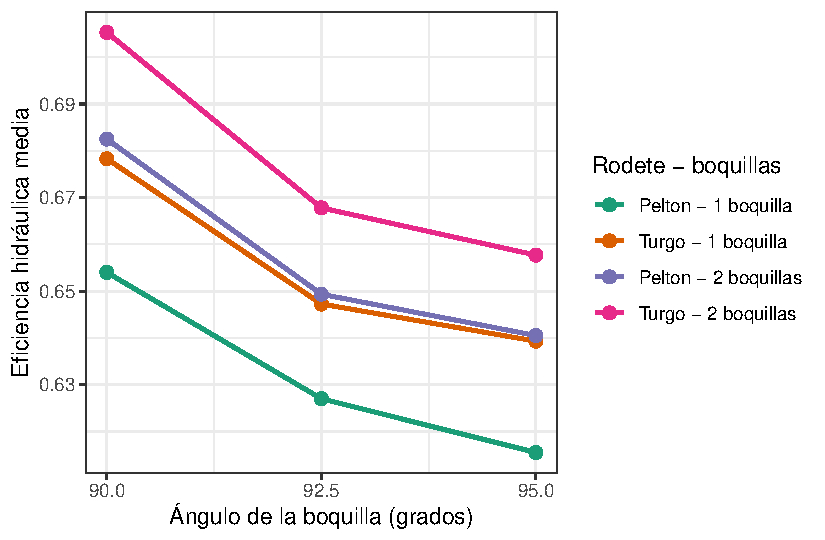
\includegraphics[width=\textwidth]{Articulo_LaTeX/Figs/perfil_angulo.pdf}\\[-2pt]
  {\small (a)}
\end{minipage}\hfill
\begin{minipage}[b]{0.49\textwidth}
  \centering
  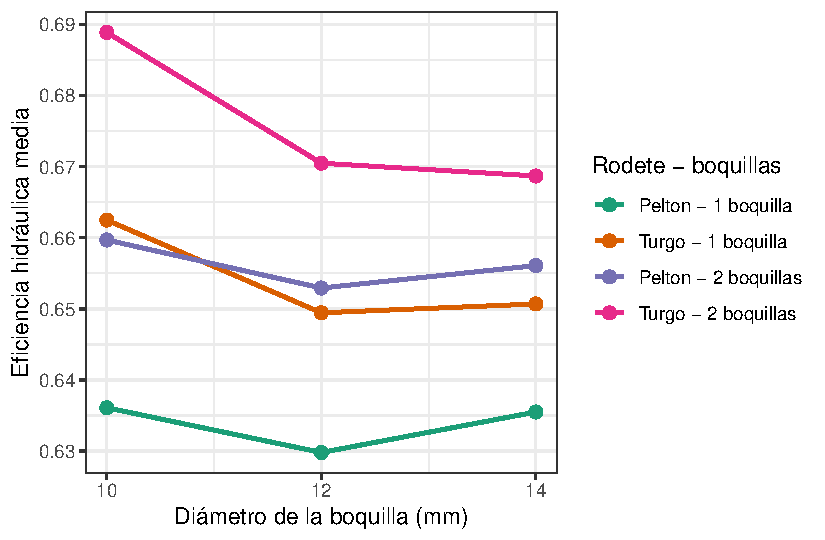
\includegraphics[width=\textwidth]{Articulo_LaTeX/Figs/perfil_diametro.pdf}\\[-2pt]
  {\small (b)}
\end{minipage}\\[6pt]
\begin{minipage}[b]{0.49\textwidth}
  \centering
  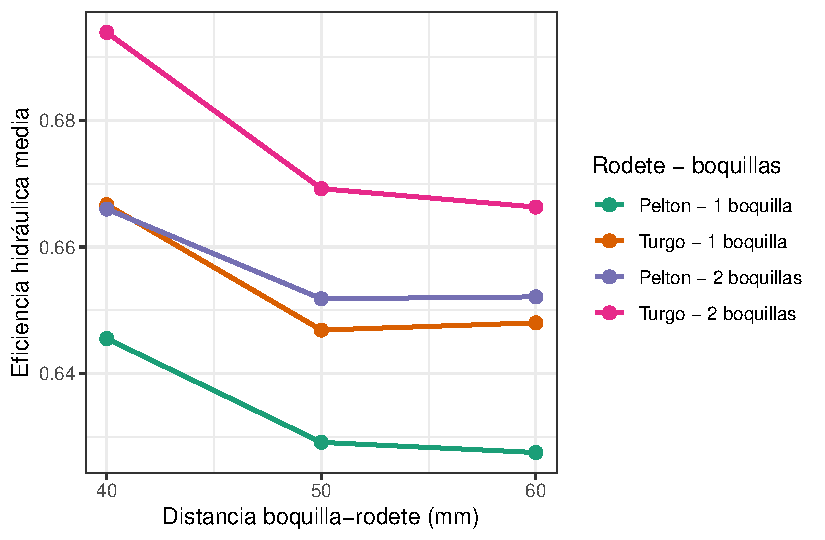
\includegraphics[width=\textwidth]{Articulo_LaTeX/Figs/perfil_distancia.pdf}\\[-2pt]
  {\small (c)}
\end{minipage}
\caption{Perfiles de la eficiencia media según el ángulo (a), el diámetro (b) y la distancia (c), para cada combinación de tipo de rodete y número de boquillas. Código: sección~7 de \texttt{anal\_descrip.R}.}
\label{fig:perfiles}
\end{figure}

Se ven tres cosas. Primero, la separación vertical entre las líneas confirma los efectos del tipo de rodete y del número de boquillas: el Turgo con dos boquillas va siempre por encima (por ejemplo, 0.7053 a 90°) y el Pelton con una boquilla siempre por debajo (0.6540 a 90°), mientras que el Turgo con una boquilla y el Pelton con dos quedan casi superpuestos en la mitad. Segundo, con el ángulo y con la distancia la eficiencia cae más del nivel bajo al nivel medio que del nivel medio al alto (en el Pelton con una boquilla, por ejemplo, pasa de 0.6540 a 0.6270 y luego a 0.6155 con el ángulo), lo que sugiere curvatura y justifica probar términos cuadráticos. Tercero, las líneas son aproximadamente paralelas, aunque con algunas diferencias de forma: con el diámetro, el Turgo con dos boquillas baja de 0.6889 a 0.6705 entre 10 y 12~mm, mientras que el Pelton con dos boquillas solo baja de 0.6597 a 0.6529. El ajuste del modelo dirá si esas diferencias corresponden a interacciones significativas.

\subsubsection{Gráfico condicional}

La Figura~\ref{fig:condicional} muestra cada corrida por separado (sección~8 del script). El eje horizontal es el ángulo y el vertical la eficiencia; los cuatro paneles separan el tipo de rodete (columnas) y el número de boquillas (filas), y el color indica el diámetro de la boquilla. Los puntos se movieron un poco en horizontal para que no se tapen entre sí. A diferencia de los gráficos anteriores, que resumen con medias, este permite ver tres variables a la vez sin promediar.

\begin{figure}[H]
\centering
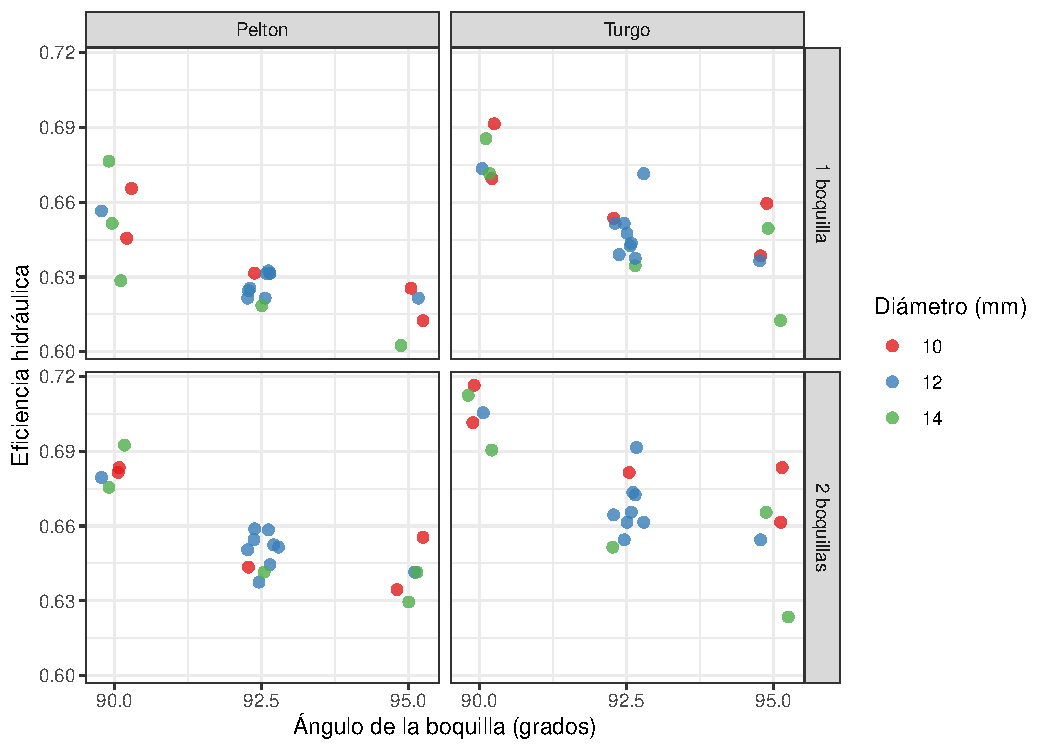
\includegraphics[width=0.85\textwidth]{Articulo_LaTeX/Figs/g5_condicional.pdf}
\caption{Eficiencia frente al ángulo de la boquilla, por tipo de rodete (columnas) y número de boquillas (filas); el color indica el diámetro. Código: sección~8 de \texttt{anal\_descrip.R}.}
\label{fig:condicional}
\end{figure}

En los cuatro paneles la eficiencia baja al pasar de 90° a 95°, así que el efecto del ángulo se repite en todas las combinaciones de rodete y número de boquillas. Los paneles de la derecha (Turgo) y los de abajo (dos boquillas) están en general más arriba, lo que coincide con lo visto en las medias. El color aporta algo nuevo: con 95° los puntos verdes (14~mm) quedan casi siempre entre los más bajos de cada panel, mientras que con 90° los tres colores están mezclados. La Tabla~\ref{tab:angulo_diametro} lo resume con las medias: con 90° la eficiencia media con 14~mm es solo 0.0058 menor que con 10~mm, pero con 95° la diferencia es de 0.0143. Es decir, el efecto del diámetro parece depender del ángulo, lo que sugiere una posible interacción entre estas dos variables.

\begin{table}[H]
\centering
\caption{Eficiencia media según el ángulo y el diámetro de la boquilla.}
\label{tab:angulo_diametro}
\begin{tabular}{lccc}
\toprule
 & \multicolumn{3}{c}{Diámetro (mm)} \\
\cmidrule(lr){2-4}
Ángulo (°) & 10 & 12 & 14 \\
\midrule
90   & 0.6819 & 0.6788 & 0.6761 \\
92.5 & 0.6525 & 0.6487 & 0.6365 \\
95   & 0.6464 & 0.6385 & 0.6321 \\
\bottomrule
\end{tabular}
\end{table}

\subsubsection{Correlaciones y matriz de dispersión}

La Tabla~\ref{tab:correlaciones} presenta las correlaciones entre la eficiencia y las variables numéricas (sección~9 del script). La correlación de Pearson mide la fuerza de la relación lineal; la de Spearman se calcula sobre los rangos de los datos y mide si la relación es monótona (siempre creciente o siempre decreciente), aunque no sea una recta. Las tres relaciones son negativas y la del ángulo es la más fuerte, lo que coincide con lo visto en las figuras anteriores. Los dos coeficientes son muy parecidos en las tres variables, lo que indica que las relaciones son monótonas y que no hay valores extremos que distorsionen la correlación de Pearson.

\begin{table}[H]
\centering
\caption{Correlación de la eficiencia con las variables numéricas.}
\label{tab:correlaciones}
\begin{tabular}{lcc}
\toprule
Variable & Pearson & Spearman \\
\midrule
Ángulo    & $-0.580$ & $-0.552$ \\
Diámetro  & $-0.132$ & $-0.137$ \\
Distancia & $-0.289$ & $-0.273$ \\
\bottomrule
\end{tabular}
\end{table}

La Figura~\ref{fig:matriz} es una matriz de dispersión que reúne todas las variables en un solo gráfico, con el Pelton en verde y el Turgo en naranja. Se lee así:
\begin{itemize}[leftmargin=*, itemsep=2pt]
  \item \textbf{Debajo de la diagonal} están los diagramas de dispersión de cada par de variables. Entre las explicativas los puntos forman una cuadrícula, porque cada una toma solo tres valores fijados por el diseño.
  \item \textbf{En la diagonal} está la densidad de cada variable para cada tipo de rodete. Las de las explicativas son prácticamente iguales en los dos rodetes, porque ambos se probaron con el mismo diseño; la de la eficiencia del Turgo está corrida hacia la derecha.
  \item \textbf{Encima de la diagonal} está la correlación de cada par, primero para todos los datos (\textit{Corr}) y luego dentro de cada rodete. Los asteriscos indican si la correlación es significativamente distinta de cero: *** para $p < 0.001$, ** para $p < 0.01$, * para $p < 0.05$ y un punto para $p < 0.1$.
  \item \textbf{La última columna} compara cada variable entre los dos rodetes con diagramas de caja, y \textbf{la última fila} muestra los histogramas por rodete.
\end{itemize}

\begin{figure}[H]
\centering
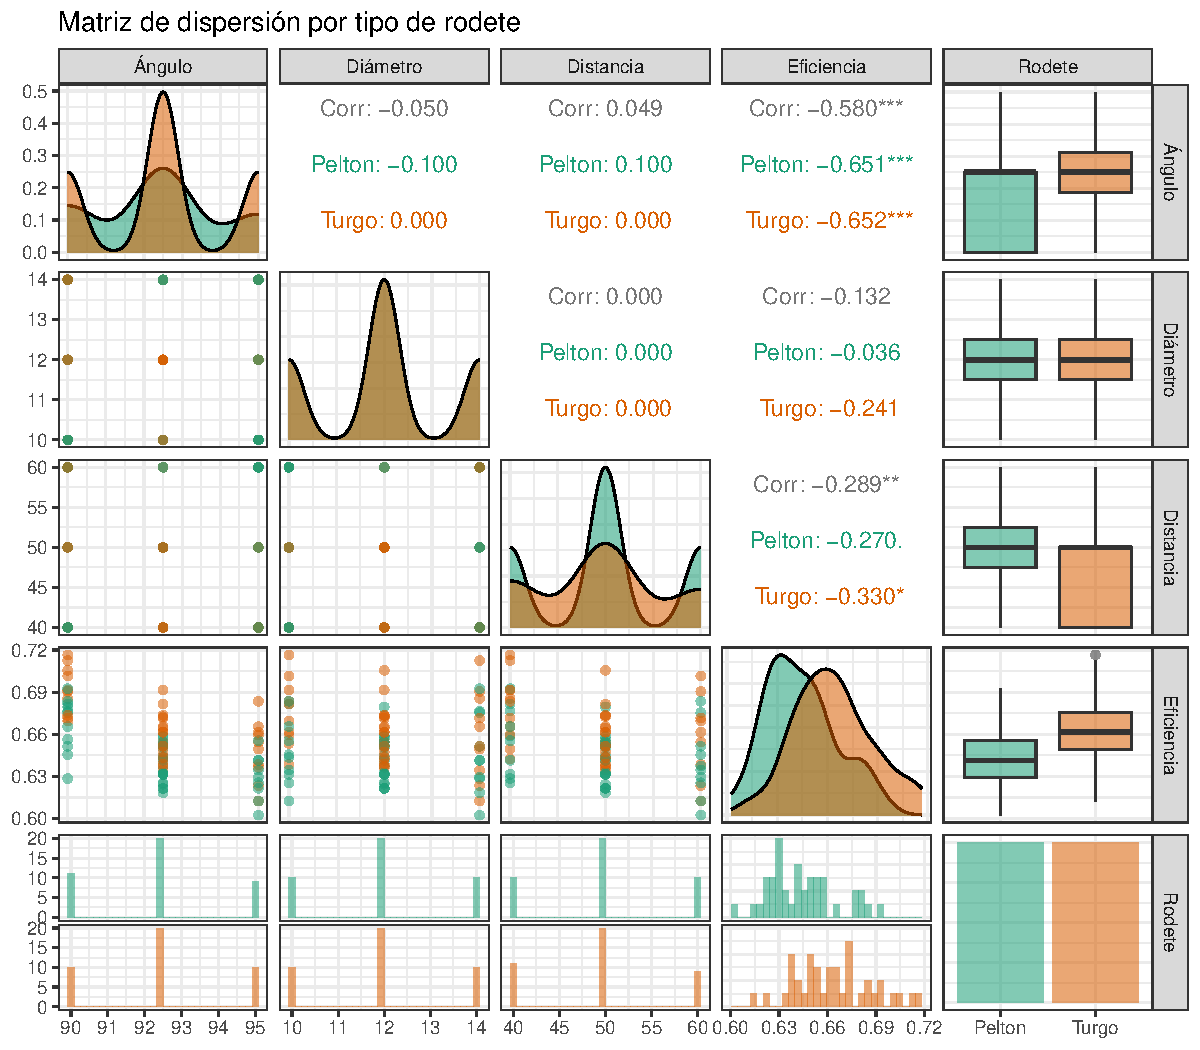
\includegraphics[width=0.9\textwidth]{Articulo_LaTeX/Figs/g6_matriz_dispersion.pdf}
\caption{Matriz de dispersión de las variables numéricas y del tipo de rodete (verde: Pelton, naranja: Turgo). Código: sección~9 de \texttt{anal\_descrip.R}.}
\label{fig:matriz}
\end{figure}

La información nueva está en las correlaciones dentro de cada rodete. La del ángulo con la eficiencia es de $-0.651$ en el Pelton y $-0.652$ en el Turgo, más fuerte que la total ($-0.580$): al juntar los dos rodetes, la diferencia de nivel entre ellos agrega variación que no tiene que ver con el ángulo y debilita la correlación. La del diámetro es casi nula en el Pelton ($-0.036$) pero de $-0.241$ en el Turgo, y la de la distancia es de $-0.270$ en el Pelton y $-0.330$ en el Turgo. Que la relación del diámetro con la eficiencia cambie según el rodete es otra señal de una posible interacción, en este caso entre el diámetro y el tipo de rodete.

Por último, entre las propias variables explicativas las correlaciones son prácticamente nulas (en valor absoluto, 0.1 o menos), tanto con todos los datos como dentro de cada rodete. Es lo que se espera en un diseño experimental, donde los investigadores fijan los valores de cada variable de forma planificada y no dejan que cambien juntas.
